\section{Performance comparison}\label{sec:performance}

We compare v3 with BAKMM-IoD only, in two independent ways that are never mixed.

\textbf{Method (a): the BAKMM-IoD paper's method.} We count the operations of each entity by running both reference
implementations with an operation counter, and multiply the counts by the average primitive times of the BAKMM-IoD paper:
$T_h$ = \ThServer\,ms on the server and \ThDrone\,ms on the Raspberry Pi~3, $T_{senc}$ = \TsencServer\,ms and
\TsencDrone\,ms. The paper does not time AES-GCM. We therefore report the AES-GCM operations separately, give the break-even
time per operation at which v3's server cost equals BAKMM-IoD's, and give one \emph{estimate}: the ratio of AES-GCM to SHA-256
time measured on our desktop (\AEADRatio), applied to the paper's $T_h$ (\AEADEst\,ms per AES-GCM operation). This estimate is
not a measurement on the paper's hardware. \Cref{tab:derivation} shows how every cost figure is derived.

\textbf{Method (b): measured.} Both implementations use the same primitive library; each run is one complete session, timed per
party, \MeasRuns\ runs on a desktop (\MeasCPU). These are desktop timings, not drone hardware.

\subsection{Computation}
\Cref{tab:comp} gives the counts. On the drone, v3 needs \DroneHashesVthree\ hash operations, $\CostDroneVthree$\,ms against
$\CostDroneBakmm$\,ms for BAKMM-IoD (\PctDrone\% lower). On the server, v3 needs \CostServerVthree\,ms of hashing and AES
($\CostServerBakmm$\,ms for BAKMM-IoD) plus \CostServerAEADops\ AES-GCM operations. v3's server cost stays at or below
BAKMM-IoD's as long as one AES-GCM operation takes at most \BreakEvenAEAD\,ms. With the estimated AES-GCM time it is
\CostServerWithAEAD\,ms (an estimate), higher than BAKMM-IoD. The retry paths cost more than a normal session and appear as
separate rows; when $MSG_2$ was lost the drone also opens the ticket with one AES-GCM decryption, shown as ``+ 1 AEAD''.
\begin{table*}[!t]
\centering
\footnotesize
\caption{Computation and communication, paper method: operations counted by the implementations' counter, times the BAKMM-IoD paper's average primitive times (Table 6 server, Table 7 Raspberry Pi 3). $T_{ae}$/$T_{ad}$: AES-128-GCM encryption/decryption, not timed by the paper and therefore not included in the ms columns.}
\label{tab:comp}
\setlength{\tabcolsep}{3pt}
\begin{tabular}{p{3.1cm}p{2.3cm}rp{3.5cm}rrr}
\toprule
Case & Drone ops & Drone ms & Server ops & Server ms & Msgs & Bits \\
\midrule
BAKMM-IoD (paper, Table 8 / Table 9) & $8T_h$ & 2.470 & $8T_h$ & 0.440 & 3 & 1792 \\
BAKMM-IoD (our implementation, counted) & $8T_h$ & 2.472 & $8T_h$ & 0.440 & 3 & 1792 \\
v3, normal session & $6T_h$ & 1.854 & $7T_h + 3T_{senc} + 2T_{ae} + 1T_{ad}$ & 0.394 + 3 AEAD & 3 & 1248 \\
v3, MSG2 lost, one retry (whole session) & $7T_h + 1T_{ad}$ & 2.163 + 1 AEAD & $7T_h + 4T_{senc} + 2T_{ae} + 1T_{ad}$ & 0.397 + 3 AEAD & 5 & 2048 \\
v3, MSG1 lost, one retry (whole session) & $7T_h$ & 2.163 & $7T_h + 3T_{senc} + 1T_{sdec} + 2T_{ae} + 1T_{ad}$ & 0.397 + 3 AEAD & 4 & 1760 \\
\bottomrule
\end{tabular}
\end{table*}

\begin{table*}[!t]
\centering
\footnotesize
\caption{Derivation of the cost figures from the BAKMM-IoD paper's average primitive times (its Tables 6--7: $T_h$, $T_{senc}$), its field sizes (Sec.~7.2) and our operation counts (\texttt{results/bench/paper\_count.json}). The AES-GCM time is an \emph{estimate}: the AES-GCM/SHA-256 time ratio measured on our desktop times the paper's $T_h$.}
\label{tab:derivation}
\setlength{\tabcolsep}{3pt}
\begin{tabular}{p{3.4cm}p{8.0cm}p{4.2cm}}
\toprule
Quantity & Derivation & Result \\
\midrule
Drone, v3 & $6\,T_h = 6 \times 0.309$ & 1.854 ms \\
Drone, BAKMM-IoD & $8\,T_h = 8 \times 0.309$ (paper: 2.47) & 2.472 ms \\
Drone reduction & $(2.47 - 1.854)/2.47$ & 24.9\% \\
Server, v3 (paper primitives) & $7\,T_h + 3\,T_{senc} = 7 \times 0.055 + 3 \times 0.003$ & 0.394 ms + 3 AEAD \\
Server, BAKMM-IoD & $8\,T_h = 8 \times 0.055$ & 0.44 ms \\
Break-even AEAD time & $(0.44 - 0.394)/3$ & 0.0153 ms \\
Server, v3, \emph{estimate} & $0.394 + 3 \times (3.429 \times 0.055)$; ratio measured on the desktop & 0.96 ms (estimate) \\
Communication, normal & v3 $576 + 416 + 256$; BAKMM-IoD $704 + 800 + 288$ & 1248 vs 1792 bits (30.4\% lower) \\
Communication, $MSG_2$ lost & $576 + 416 + 512 + 288 + 256$ ($MSG_1, MSG_2, MSG_{1r}, MSG_{2r}, MSG_3$) & 2048 bits \\
Communication, $MSG_1$ lost & $576 + 512 + 416 + 256$ ($MSG_1, MSG_{1r}, MSG_2, MSG_3$) & 1760 bits \\
Drone storage & v3 160 + 96 + 256; BAKMM-IoD 160 + 256 + 256 + 256 & 512 vs 928 bits (44.8\% lower); v3 up to 832 with $N_1, N_{1r}$ \\
Server storage per drone & v3 256 + 128 + 96 + 256 + 128 + 128 + 160 + 128; BAKMM-IoD 160 + 256 + 256 & 1280 vs 672 bits \\
Server, own secrets & field by field (\cref{tab:storage}) & 128 vs 512 bits \\
Server storage, $n$ drones & per drone $\times n$ + own & v3 $1280n + 128$; BAKMM-IoD $672n + 512$ bits \\
\bottomrule
\end{tabular}
\end{table*}


\subsection{Communication}
\Cref{tab:comm} counts bits with the paper's field sizes. A normal v3 session takes three messages and \BitsVthree\ bits
against \BitsBakmm\ (\PctBits\% lower). A retry adds $MSG_{1r}$ and, if $MSG_2$ was lost, $MSG_{2r}$: a session with
$MSG_2$ lost and one retry takes \MsgsRetryLostTwo\ messages and \BitsRetryLostTwo\ bits, more than BAKMM-IoD
(\cref{fig:comm-cases}). BAKMM-IoD has no retry mechanism, so it has no value for the lost-message cases.
\begin{table*}[!t]
\centering
\footnotesize
\caption{Communication cost in bits, with the field sizes of the BAKMM-IoD paper (Sec.~7.2).}
\label{tab:comm}
\setlength{\tabcolsep}{3pt}
\begin{tabular}{lrrp{4.3cm}}
\toprule
Message & BAKMM-IoD & v3 & v3 fields (bits) \\
\midrule
MSG1 & 704 & 576 & TID 160 + N1 160 + V1 256 \\
MSG2 & 800 & 416 & N2 160 + V2 256 \\
MSG3 & 288 & 256 & V3 256 \\
total & 1792 & 1248 &  \\
MSG1r (retry only) & -- & 512 & PID 96 + N1r 160 + V1r 256 \\
MSG2r (retry only) & -- & 288 & T 160 + tag 128 \\
\bottomrule
\end{tabular}
\end{table*}

\begin{figure}[!htbp]
\centering
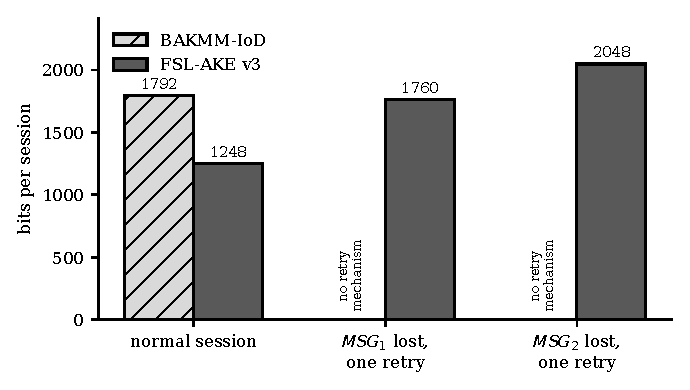
\includegraphics[width=0.62\textwidth]{figures/graph_comm_cases.pdf}
\caption{Communication per session in bits, field sizes of the BAKMM-IoD paper (Sec.~7.2), for a normal session and for one
retry after a lost $MSG_1$ or $MSG_2$ (\texttt{results/bench/paper\_count.json}; generated by
\texttt{paper/scripts/make\_graphs.py}).}
\label{fig:comm-cases}
\end{figure}

\subsection{Storage}
\Cref{tab:storage} counts stored bits field by field. The drone stores \StoreDroneVthree\ bits against \StoreDroneBakmm\
(\PctStoreDrone\% lower), up to \StoreDroneVthreeMax\ while it waits for an answer. The server's own secrets take
\StoreOwnVthree\ bits against \StoreOwnBakmm. Per drone, however, the server stores \StoreServerVthree\ bits against
\StoreServerBakmm: BAKMM-IoD keeps $RID_{DE}$ and $MS$ in clear (the cause of F8), while v3 keeps encrypted indices, an
authenticated record and the retry ticket.
\begin{table*}[!htbp]
\centering
\footnotesize
\caption{Storage per entity, field by field, same counting rule for both schemes.}
\label{tab:storage}
\setlength{\tabcolsep}{3pt}
\begin{tabular}{p{1.6cm}lp{9.6cm}r}
\toprule
Entity & Scheme & Stored fields (bits) & Total \\
\midrule
drone & BAKMM-IoD & TID\_DE 160, RID\_DE 256, TC\_DE 256, MS\_DE-ES 256 & 928 \\
drone & v3 & TID 160, PID 96, K 256 & 512 \\
server per drone & BAKMM-IoD & TID\_DE 160, RID\_DE 256, MS\_DE-ES 256 & 672 \\
server per drone & v3 & I(TID): 2 AES blocks 256, I(PID): 1 AES block 128, record nonce nu 96, C = AEAD(K): ciphertext 256, C: tag 128, ticket index I(PID\_old): 1 AES block 128, ticket T: ciphertext of N2 160, ticket T: tag 128 & 1280 \\
server own & BAKMM-IoD & RID\_ES 256, TC\_ES 256 & 512 \\
server own & v3 & X\_ES 128 & 128 \\
\bottomrule
\end{tabular}
\end{table*}


\textbf{Growth with the number of drones.} The cost of one session is a constant number of operations per party in both
schemes ($O(1)$ per session), independent of the number of drones. Server storage grows linearly with the number $n$ of
registered drones: $\StoreServerVthree n + \StoreOwnVthree$ bits for v3 against $\StoreServerBakmm n + \StoreOwnBakmm$ bits
for BAKMM-IoD (\cref{fig:storage-n}). Our server implementation (\texttt{impl/server.py}) finds a record by its index $I(TID)$
or $I(PID)$ in a hash table (a Python dictionary), which takes expected constant time per lookup; the BAKMM-IoD paper does not
state its lookup structure.
\begin{figure}[!htbp]
\centering
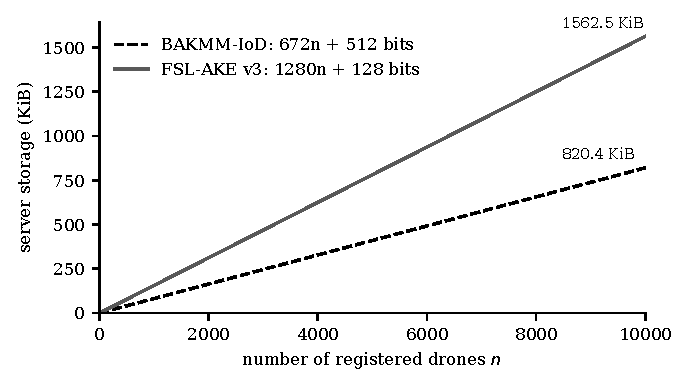
\includegraphics[width=0.62\textwidth]{figures/graph_storage_n.pdf}
\caption{Server storage against the number of registered drones $n$, from the field-by-field counts of \cref{tab:storage}
(per-drone bits $\times\, n$ + the server's own secrets); generated by \texttt{paper/scripts/make\_graphs.py}.}
\label{fig:storage-n}
\end{figure}

\subsection{Measured timings}
\Cref{tab:measured} gives the desktop measurements. The median drone time is \MeasDroneVthree\,ms for v3 and
\MeasDroneBakmm\,ms for BAKMM-IoD; the median server time is \MeasServerVthree\,ms for v3 and \MeasServerBakmm\,ms for
BAKMM-IoD, higher for v3. \Cref{fig:timing-box} shows the distribution of the \MeasRuns\ runs per party.
\begin{table}[!htbp]
\centering
\footnotesize
\caption{Measured time per session per party in ms, 1000 runs after 50 warm-up, on a desktop (13th Gen Intel(R) Core(TM) i7-1360P, Python 3.12.0, cryptography 46.0.7). These are desktop timings, not drone hardware. Computed from the per-run files \texttt{results/timing/raw\_*.csv} (run of 2026-10-19).}
\label{tab:measured}
\setlength{\tabcolsep}{3pt}
\begin{tabular}{llrrrrr}
\toprule
Scheme & Party & Mean & Median & Std dev & Min & Max \\
\midrule
BAKMM-IoD & drone & 0.0353 & 0.0349 & 0.0186 & 0.0224 & 0.5140 \\
BAKMM-IoD & server & 0.0351 & 0.0350 & 0.0132 & 0.0226 & 0.2245 \\
v3 & drone & 0.0232 & 0.0192 & 0.0315 & 0.0156 & 0.9774 \\
v3 & server & 0.0661 & 0.0578 & 0.0239 & 0.0478 & 0.3293 \\
\bottomrule
\end{tabular}
\end{table}

\begin{figure}[!htbp]
\centering
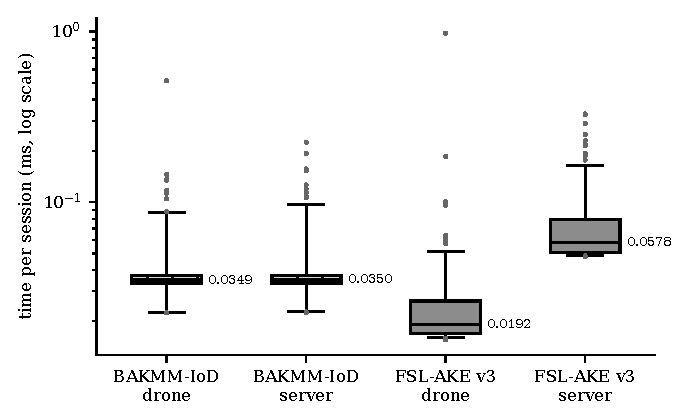
\includegraphics[width=0.62\textwidth]{figures/graph_timing_box.pdf}
\caption{Measured time per session and party, \MeasRuns\ runs after \MeasWarmup\ warm-up runs (\texttt{results/timing/raw\_*.csv});
boxes: quartiles, line and label: median, whiskers: 1st and 99th percentile, dots: runs outside them; log scale. Desktop
(\MeasCPU, Python \MeasPython, cryptography \MeasCrypto), not drone hardware. Generated by \texttt{paper/scripts/make\_graphs.py}.}
\label{fig:timing-box}
\end{figure}

\subsection{Summary}
\Cref{tab:final-cost} lists every quantity with its method and \cref{fig:charts} plots the main ones. v3 is lightweight on the
drone side and has lower communication in a normal session; it stores more per drone on the server, and its server time is
lower only if AES-GCM is at most \BreakEvenAEAD\,ms per operation: with the estimated AES-GCM time (estimate
\CostServerWithAEAD\,ms) and on measured desktop timings (\MeasServerVthree\ versus \MeasServerBakmm\,ms) it is higher.
\begin{table*}[!t]
\centering
\footnotesize
\caption{Cost summary, every quantity, including those where v3 is higher.}
\label{tab:final-cost}
\setlength{\tabcolsep}{3pt}
\begin{tabular}{p{3.6cm}rrrp{1.6cm}p{5.6cm}}
\toprule
Quantity & BAKMM-IoD & v3 & Diff. & Result & Method \\
\midrule
drone time, ms & 2.47 & 1.854 & -0.616 & \textbf{v3 lower} & paper method: our operation count x paper Table 7 (RPi 3) \\
server time, ms (paper primitives only) & 0.44 & 0.394 & -0.046 & \textbf{v3 lower} & paper method: our count x paper Table 6 \\
server time, ms (with estimated AES-GCM) & 0.44 & 0.96 & 0.52 & \textbf{v3 HIGHER} & paper method + AES-GCM time = desktop-measured ratio t(GCM)/t(SHA-256) x paper T\_h (estimate) \\
drone time, ms (measured median) & 0.0349 & 0.0192 & -0.0157 & \textbf{v3 lower} & measured: desktop (13th Gen Intel(R) Core(TM) i7-1360P), 1000 runs; not drone hardware \\
server time, ms (measured median) & 0.035 & 0.0578 & 0.0228 & \textbf{v3 HIGHER} & measured: desktop (13th Gen Intel(R) Core(TM) i7-1360P), 1000 runs \\
communication, bits per session & 1792 & 1248 & -544 & \textbf{v3 lower} & field lengths of the paper's Sec. 7.2 \\
drone storage, bits & 928 & 512 & -416 & \textbf{v3 lower} & field by field (paper\_count.json) \\
server storage per drone, bits & 672 & 1280 & 608 & \textbf{v3 HIGHER} & field by field \\
server own secrets, bits & 512 & 128 & -384 & \textbf{v3 lower} & field by field \\
\bottomrule
\end{tabular}
\end{table*}

\def\ChartDrone{(BAKMM-IoD,2.47) (v3,1.854)}
\def\ChartServer{(BAKMM-IoD,0.44) (v3,0.394)}
\def\ChartServerAEAD{(BAKMM-IoD,0.44) (v3,0.96)}
\def\ChartBits{(BAKMM-IoD,1792) (v3,1248)}
\def\ChartStoreDrone{(BAKMM-IoD,928) (v3,512)}
\def\ChartStoreServer{(BAKMM-IoD,672) (v3,1280)}

\begin{figure}[!htbp]
\centering
\begin{tikzpicture}
\begin{groupplot}[group style={group size=3 by 1, horizontal sep=1.4cm}, width=4.8cm, height=4.6cm, ybar, /pgf/bar width=0.55cm, enlarge y limits={upper, value=0.18},
  symbolic x coords={BAKMM-IoD,v3}, xtick=data, ymin=0, enlarge x limits=0.6, nodes near coords, every node near coord/.append style={font=\footnotesize, /pgf/number format/precision=3, /pgf/number format/1000 sep={}},
  tick label style={font=\footnotesize}, label style={font=\footnotesize}, title style={font=\small}]
\nextgroupplot[title={Drone computation}, ylabel={ms (paper method)}] \addplot[fill=accent!70] coordinates {\ChartDrone};
\nextgroupplot[title={Communication}, ylabel={bits per session}] \addplot[fill=accent!70] coordinates {\ChartBits};
\nextgroupplot[title={Server storage}, ylabel={bits per drone}] \addplot[fill=black!35] coordinates {\ChartStoreServer};
\end{groupplot}
\end{tikzpicture}
\caption{BAKMM-IoD versus v3: drone computation (paper method), communication (normal session) and server storage per drone.
The first two panels, where v3 is lower, are drawn in blue; the third, where v3 is higher, in grey.}
\label{fig:charts}
\end{figure}
